\documentclass[a4paper,12pt]{article}

% Packages
\usepackage[dutch]{babel}           
\usepackage[latin1]{inputenc}       	% speciale karakters
\usepackage{graphicx} 					% figuren

\usepackage{enumitem}
\usepackage{longtable}
\usepackage{array}
\usepackage[hyphens]{url}
\usepackage{pdfpages}
\usepackage{amssymb}
\usepackage{fullpage}
\usepackage{amsmath}
\usepackage{graphicx}
\usepackage[font=small,format=plain,labelfont=bf,up,textfont=it,up]{caption}
\usepackage{float}
\usepackage[bottom]{footmisc}
\usepackage[T1]{fontenc}
\usepackage{lastpage}
\usepackage{fancyhdr}
\usepackage{caption}
\usepackage{subcaption}
\usepackage{varioref}
\usepackage{hyperref}

% schema's wijzigen door als .eps te exporteren, latex maakt zelf pdf versie
% aan die hij gebruikt
\usepackage{epstopdf}

\author{Tom Naessens, Enver Bral, Cynric Huys en Felix Van der Jeugt}

\setlength{\parskip}{1ex}
\setlength{\parindent}{0ex}

\begin{document}

\begin{titlepage}

\fontsize{12pt}{14pt}
\selectfont

\begin{center}

\begin{figure}[htb]
\centering
\renewcommand{\tabcolsep}{5pt}
\renewcommand{\arraystretch}{0}
  \begin{tabular}{@{}cc@{}}
    \includegraphics[width=.3\textwidth]{includes/img/ugent-logo}
  \end{tabular}
\end{figure}

\vspace{0.5cm}

Faculty of Engineering\\
Master of Science in Computer Science\\

\vspace{3.5cm}

\fontseries{bx}
\fontsize{17.28pt}{21pt}
\selectfont

\hrule
\vspace{10pt}
\textsc{Project Informatiebeveiliging:\\ Beveiliging voor elektronisch stemmen via het Web}\\
\vspace{10pt}
\hrule

\vspace{25pt}

\fontseries{m}
\fontsize{12pt}{14pt}
\selectfont

\vspace{6cm}

\fontseries{m}
\fontsize{12pt}{14pt}
\selectfont

\hspace{0.5cm}
\textbf{ \textsc{
	Begeleiders: \hfill Groep 1:\\
	Prof. Eric Laermans \hfill Enver Bral (ICT)\\
	Prof. Tom Dhaene \hfill Cynric Huys (SE)\\
	\hfill Tom Naessens (SE)\\
	\hfill Felix Van der Jeugt (MWI)\\
}}
\end{center}
\end{titlepage}


\section{Initi\"ele idee\"en}

De basisprincipes van elke mogelijk oplossing voor het gegeven probleem zijn
hetzelfde. We willen iedereen verplichten om anoniem \'e\'en enkele stem uit te
brengen. Direct uit deze stelling volgt de grootste uitdaging: enerzijds wil
je mensen anoniem laten stemmen, maar anderzijds moet je ieders identiteit wel
kennen om te kunnen controleren of men wel gestemd heeft.

De andere problemen en vereisten die zich voordoen zijn slechts te verwachten.
We eisen vertrouwelijkheid van de stem, authenticatie, verbieden van dubbel
stemmen, etc...

Hieronder maken we een opsomming van de verschillende idee\"en die we hebben
bedacht om dit probleem op te lossen. Bij elke oplossing vermelden we een aantal
voor- en nadelen. Onze uiteindelijke keuze vindt u dan terug in de volgende
sectie, samen met een motivatie.

\subsection{Vereiste beveiligingsfuncties}

Hieronder lijsten we de verschillende vereiste beveiligingsfuncties op, samen
met de reden waarom wij denken dat deze aanwezig moeten zijn in het systeem.

\textbf{Vertrouwelijkheid} Wanneer men een stem uitbrengt verwacht men dat
dit anoniem gebeurt. Men wil niet dat na het stemmen een specifieke stem kan
verbonden worden met de persoon die deze stem heeft uitgebracht. Zoals later zal
blijken zal deze voorwaarde voor heel wat problemen zorgen.

\textbf{Authenticatie} Enerzijds wil men, wanneer men een \emph{ingevulde
stembrief} ontvangt, kunnen controleren dat de persoon die deze brief indient
niet reeds een stem heeft uitgebracht. Hiertoe zal de identiteit van deze
persoon moeten kunnen worden bepaald. Men wil dus bij het ontvangen van een
stembrief zeker zijn dat het om een persoon is die nog niet gestemd heeft en
dat die persoon is wie hij/zij beweert te zijn. Anderzijds wil de persoon die
zijn stem uitbrengt kunnen verifi\"eren dat de stem wordt ingediend bij een
betrouwbare identiteit (stembus) en dus niet in verkeerde handen terechtkomt
(zoals iemand die de stem wil inkijken -- of zelfs aanpassen).

\textbf{Toegangscontrole} Het is de bedoeling dat niemand een \emph{stembus} kan
inkijken tot na het einde van de indienperiode. Indien dit niet gegarandeerd
zou worden zou men de stembrief kunnen inkijken telkens iemand een stem maakt
en dus zo te weten komen wat iedere persoon gestemd heeft. Daarnaast is het de
bedoeling dat niemand de stemmen kan aanpassen of verwijderen wanneer deze zich
in de \emph{stembus} bevinden, noch wil men dat personen die reeds een stem
hebben uitgevoerd een stem kunnen toevoegen aan de \emph{stembus}.

\textbf{Data-integriteit} Er zal zekerheid moeten zijn dat als een stembrief
opgestuurd wordt naar de stembus, dat deze brief daar effectief toekomt en dat
deze onder weg niet aangepast werd. Een bepaalde partij zou er bijvoorbeeld
baat bij hebben mochten de stemmen aangepast worden zodat ze niet tegen maar
net voor deze partij zou stemmen, of dat stemmen in het nadeel van deze partij
de stembus nooit bereiken. Het is verder ook niet de bedoeling dat een stem
meer dan \'e\'en keer kan ingediend worden, anders zou men meerdere stemmen ten
voordele van zichzelf kunnen indienen.

\textbf{Onweerlegbaarheid} Het is belangrijk bij te houden wie zijn/haar
stem heeft uitgebracht en wie niet. Aangezien in Belgi\"e stemplicht geldt,
staat er een straf op het niet uitbrengen van een stem. Wanneer een stem
ingezonden wordt, wil men dus graag een bewijs dat men effectief een stem heeft
uitgebracht, anders zou men achteraf het tegendeel kunnen beweren en is men (ten
onrechte) verplicht een boete te betalen.

\textbf{Beschikbaarheid} Op de verkiezingsdag verwacht men zijn stem te kunnen
uitbrengen binnen de daarvoor opgestelde uren. Het is dus niet de bedoeling
dat men voor gesloten deuren komt te staan of dat de \emph{stembus} tijdelijk
onbeschikbaar is. Merk op dat we hiermee geen verdere rekening houden in dit
project, we gaan er vanuit dat de overheid genoeg kennis en geld heeft om dit te
voorzien.

\subsection{Voorstel 1: Afgehaalde stembrieven tellen}

Met ons eerste idee proberen we zo goed mogelijk de normale verkiezingen na te
bootsen. Daarbij zal je eerst een stembrief afhalen en je identiteit aantonen.
Vervolgens breng je je stem uit op deze brief. De brief, waarmee de identiteit
van de stemmer niet te achterhalen is, wordt vervolgens gedeponeerd in een
stembus.

Bij onze gedachtegang vervangen we de bijzitters door een vertrouwde derde. Het
vertrouwen in deze derde kan verkregen worden door er een open source server van
te maken.

De stembus wordt dan vervangen door een telserver die de overheid beheert.

Het proces is ge\"illustreerd in Figuur \ref{fig:voorstel1} en verloopt als
volgt. De stemmer identificeert zich bij de bijzitter (1). Hij krijgt een
stembrief in de vorm van een (persoonlijke) symmetrische sleutel, de echte brief
(lijst met politici/partijen) en een anonieme identifier (2). De stemmer vult de
brief in, encrypteert deze met de symmetrische sleutel en voegt de identifier
toe. Dit pakket wordt naar de overheid verzonden (3). Zij vragen de symmetrische
sleutel (5) aan de bijzitters met behulp van de identifier (4) en kunnen zo de
stem decrypteren zonder de werkelijke identiteit te kennen. De bijzitter kan
controleren of iedereen stemt omdat de overheid elke binnengekregen identiteit
aan hen zal melden (4).

\begin{figure}
  \centering
  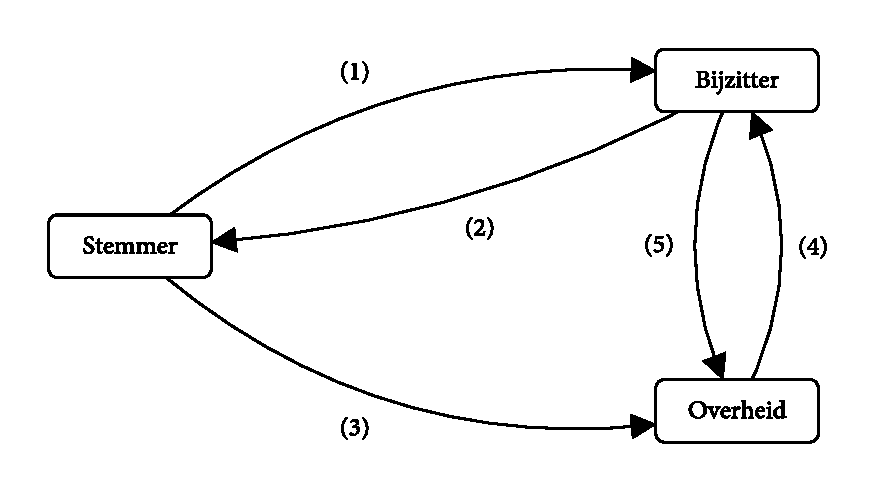
\includegraphics[width=0.8\textwidth]{includes/img/schema_voorstel1.eps}
  \caption{Voorstel 1: Afgehaalde stembrieven tellen.}
  \label{fig:voorstel1}
\end{figure}

Dit voorstel voldoet aan de principes:

\begin{description}
    \item[Vertrouwelijkheid] Op voorwaarde dat de vertrouwde derde effectief
      betrouwbaar is, is dit criterium voldaan. De overheid kan niet achterhalen
      van wie de stem komt, tenzij ze je IP-adres onderzoeken. Dit laatste
      kunnen we echter omzeilen door tussen de stemmer en de overheid een proxy
      te plaatsen, dit idee wordt later nog verder uitgewerkt.
    \item[Authenticatie] Wordt voorzien door de bijzitter.
    \item[Toegangscontrole] Zolang de overheid de stemmen niet inkijkt, aanpast
      of verwijdert voor het einde van de verkiezingsdag is dit voldaan. In de
      praktijk kan dit echter problemen vormen aangezien deze systemen
      waarschijnlijk live gemonitord moeten worden. Inkijken vormt echter geen
      probleem aangezien stemmen niet aan personen kunnen gelinkt worden. Het
      aanpassen en verwijderen mag echter niet kunnen gebeuren.
    \item[Data-integriteit] De stembrief kan onderweg van de bijzitter naar de
        stemmer getekend worden, naast encryptie. Van de bijzitter naar de
        overheid kan een hash meegegeven worden.
    \item[Onweerlegbaarheid] De stemmer moet een getekend bewijsje van de
        bijzitter kunnen krijgen dat hij gestemd heeft.
    \item[Beschikbaarheid] Onze servers moeten beschikbaar zijn en blijven
      tijdens de stemperiode.
\end{description}

Willen we nog meer vertrouwelijkheid, en dus het IP-adres van de stemmer ook
geheim houden voor de overheid, zullen we een extra proxy, de stembus, tussen de
stemmer en de overheid sturen. Deze geeft gewoon letterlijk alle verkeer door
van de stemmer naar de overheid en omgekeerd, maar haalt dus het IP er af.

\subsection{Voorstel 2: Geneste enveloppen}

Voor ons tweede idee kunnen we de analogie trekken met een enveloppe in een
enveloppe. We sturen als het ware geheime data die op brief is neergeschreven in
een bepaalde enveloppe. Deze data moet echter langs een andere entiteit (zoals
de post) passeren die extra data nodig heeft die geheim moet blijven voor de
buitenwereld, maar die de uiteindelijke inhoud van de brief niet mag zien. Het
idee is om de enveloppe samen met die extra data in een andere enveloppe te
steken. De post zal dan de buitenste enveloppe openen om de extra data te
verkrijgen alvorens de binnenste enveloppe terug op te sturen.

Als we dit nu doortrekken naar ons specifieke probleem rond stemmen, dan kunnen
we opnieuw drie partijen identificeren: de stemmer, de bijzitter en de overheid.
Het is opnieuw de bedoeling dat de bijzitter enkel bijhoudt wie gestemd heeft en
dat de overheid de uiteindelijke stemtelling doet, zonder te weten wie waarvoor
gestemd heeft.

\begin{figure}
  \centering
  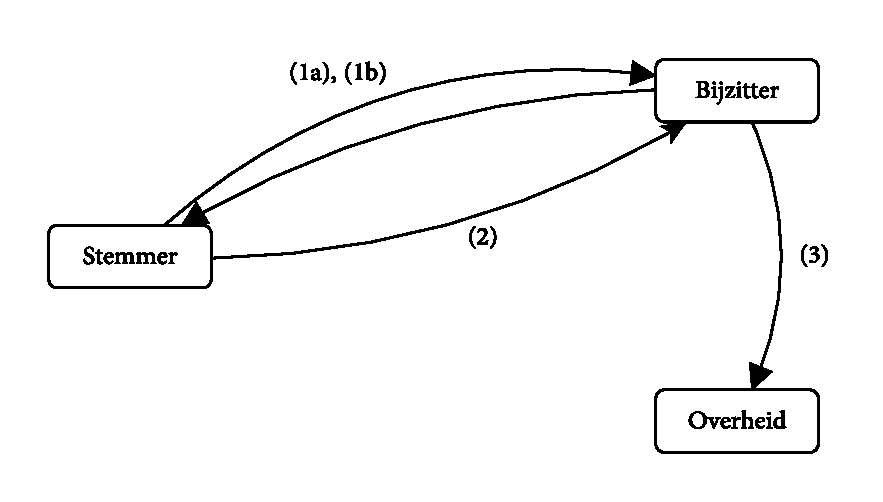
\includegraphics[width=0.8\textwidth]{includes/img/schema_voorstel2.eps}
  \caption{Voorstel 2: Geneste enveloppen.}
  \label{fig:voorstel2}
\end{figure}

We kunnen het stemmen nu uitvoeren als volgt en zoals ge\"illustreerd in Figuur
\ref{fig:voorstel2}. We doen eerst een initi\"ele communicatie met de bijzitter
zodat we zowel zijn publieke sleutel als die van de overheid te weten komen
(b.v. door authenticatie via de bijzitter's certificaat, dat getekend is door de
overheid) (1a). Vervolgens vragen wij een lijst van mogelijke partijen/politici
waarop we kunnen stemmen aan de bijzitter en voeren onze stem uit (1b). Voor
het verzenden encrypteren wij de stem met een sleutel die enkel gedecrypteerd
kan worden door de overheid zoals zijn publieke sleutel of, als het om veel
data gaat, een symmetrische sleutel die door communicatie met asymmetrische
encryptie wordt doorgegeven. Vervolgens voegen wij de unieke identifier voor
deze user toe aan dit bericht en encrypteren dit geheel met een sleutel die
enkel gedecrypteerd kan worden door de bijzitter. Hier hebben we dus als het
ware een enveloppe in een enveloppe. Als we dit geheel sturen naar de bijzitter
(2), kan deze ons identificeren door de buitenste laag te decrypteren. Deze
weet dus dat wij een stem hebben uitgebracht en kan de binnenste brief verder
doorsturen naar de overheid (3). Vervolgens kan de overheid als enige deze data
decrypteren en zo de stem van de gebruiker te weten komen, zonder dat hij zijn
identiteit weet (deze data is namelijk reeds verwijderd bij het passeren bij de
bijzitter).

Voldoening aan de beveiligingsfuncties:

\begin{description}
    \item[Vertrouwelijkheid] Aangezien enkel de overheid de eigenlijke stem kan
    decrypteren, en de identeit van de gebruiker niet wordt meegegeven aan de
    overheid, is dit voldaan.
    \item[Authenticatie] Wordt opnieuw voorzien door de bijzitter.
    \item[Toegangscontrole] Zelfde opmerking als in voorstel 1.
    \item[Data-integriteit] Voldaan indien alle berichten getekend worden door
      de verzenders. Indien de stem van de stemmer verwijderd wordt, zal de
      stemmer later in het proces hiervan op de hoogte gesteld worden door het
      feit dat hij geen ontvangstbewijs heeft ontvangen/kan opvragen. De stem
      zou dan dus opnieuw verzonden kunnen worden.
    \item[Onweerlegbaarheid] De stemmer moet een getekend bewijsje van de
        bijzitter krijgen dat hij gestemd heeft.
    \item[Beschikbaarheid] Onze servers moeten beschikbaar zijn en blijven
      tijdens de stemperiode.
\end{description}

Merk hier echter op dat we de \emph{bijzitter} compleet vertrouwen om als proxy
te fungeren. Mocht de bijzitter namelijk andere zaken doen dan de hierboven
besproken stappen, dan bevindt deze zich in de perfecte positie om een soort
\emph{man-in-the-middle} aanval te kunnen uitvoeren. Hij zou zich zowel kunnen
voordoen als de overheid (ten opzichte van de stemmer) en als een stemmer (ten
opzichte van de overheid) om in naam van de stemmer zijn eigen stemmer uit te
brengen. Deze methode vereist dus een compleet vertrouwen in de software die
achter de \emph{bijzitter} zit. Om dit vertrouwen te garanderen stellen wij dan
ook voor deze server open source te maken.

\section{Verkozen idee}

Uiteindelijk hebben wij ervoor gekozen om het eerste voorstel verder uit te
werken en wel om twee redenen. Ten eerste geeft het idee beter weer wat de
verschillende verantwoordelijkheden van de verschillende entiteiten zijn, en
zijn hun verantwoordelijkheden beter verdeeld. Ten tweede hebben wij niet het
probleem dat, indien de bijzitter niet 100\% vertrouwd wordt, deze eventuele
ongewenste wijzigingen aan de uitgevoerde stemmen zou kunnen aanbrengen.  In wat
volgt zal dit eerste idee dan ook wat meer in detail uitgewerkt worden.

\section{Verdere uitwerking}

We hebben ervoor gekozen om in plaats van een webbrowser een Java-applicatie als
client te gebruiken. Dit omdat we op deze manier eenvoudiger encryptie kunnen
toepassen en ook meer controle hebben over wat er precies verstuurd wordt naar
de servers. Merk verder op dat we de entiteit \emph{stembus}, die in feite als
simpele proxy fungeert, zullen weglaten aangezien we er hier kunnen van uit gaan
dat de \emph{overheid} niet zal proberen te achterhalen wat de identiteit is van
de gebruiker die een stem heeft uitgebracht. Mocht de overheid niet te
vertrouwen zijn voegt deze functie enkel meer complexiteit toe: het is maar een
kleine stap voor de corrupte overheid om logs bij te houden op deze
proxyserver.

De verschillende stappen in het stem-proces worden hieronder kort opgelijst en
iedere stap zal in de volgende secties in meer detail behandeld worden.

\begin{enumerate}
  \item De stemmer verkrijgt een lege stembrief van de bijzitter.
  \item De stemmer dient de stembrief in bij de overheid.
  \item De stemmer verkrijgt een getekend bewijs dat hij/zij gestemd heeft.
\end{enumerate}

\begin{figure}
  \centering
  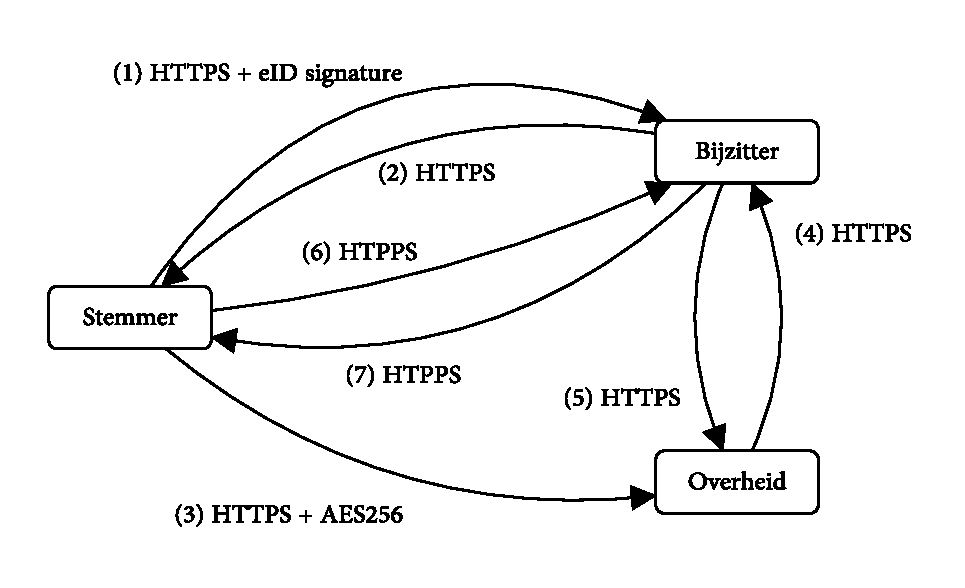
\includegraphics[width=0.8\textwidth]{includes/img/schema_ontwerp.eps}
  \caption{Verkozen architectuur: Afgehaalde stembrieven tellen.}
\end{figure}

\subsection{De stemmer verkrijgt een lege stembrief van de bijzitter}

Wanneer de stemmer de applicatie start, kan hij een stemformulier aanvragen.
Hiervoor wordt de elektronische identiteitskaart gebruikt. Eerst wordt het
rijksregisternummer van de persoon opgevraagd.  Dit nummer zal fungeren als een
unieke identifier voor de gebruiker. Indien de gebruiker vervolgens de correcte
pincode ingeeft, zal deze identifier getekend worden met de private sleutel van
de identiteitskaart. Merk op dat dit tekenen enkel kan gebeuren door personen
die zowel de identiteitskaart als de pincode bezitten. Vervolgens worden beide
zaken doorgestuurd naar de bijzitter (1).  Dit doorsturen gebeurt in een
POST-request over een HTTPS-connectie, zodat vertrouwelijkheid en authenticatie
van de bijzitter gegarandeerd is.

De bijzitter kan dan, gebruik makend van de public key infrastructure van de
overheid, bevestigen dat de gebruiker beweert wie hij is te zijn. Daarnaast
wordt er ook gecontroleerd of deze gebruiker reeds gestemd heeft of niet. Indien
niet, wordt een random gegenereerde (32 byte), \emph{anonieme} identifier
toegekend aan deze gebruiker en wordt er een symmetrische sleutel gegenereerd
die uniek is voor deze gebruiker. Deze sleutel wordt op een random manier
gegenereerd en zal later gebruikt worden als AES-256 sleutel.  De POST-request
wordt dan beantwoord met deze informatie, alsook de lijst van partijen en
personen waarop gestemd kan worden (een \emph{lege stembrief} als het ware)
(2).

\subsection{De stemmer dient de stembrief in bij de overheid}

Nadat de stemmer de lege stembrief heeft ontvangen, kan hij zijn eigenlijke
stem uitvoeren. Hij maakt zijn selectie van de partij en personen waar hij op
stemt. Daarna wordt deze data ge\"encrypteerd met AES-256 waarbij als sleutel de
symmetrische sleutel die eerder door de bijzitter verstuurd was wordt gebruikt.
Deze ge\"encrypteerde data wordt samen met de \emph{anonieme} identifier
doorgestuurd in een POST-request over HTTPS naar de overheid (3). Opnieuw werd
hier HTTPS gekozen mede voor de authenticatie van de overheidsserver (op basis
van een certificaat) en vertrouwelijkheid.

De overheid zal bij het ontvangen van dit bericht de eigenlijke stem moeten
decrypteren, maar kent de geheime sleutel niet. Hiervoor wordt een POST-request
naar de bijzitter gestuurd, opnieuw over HTTPS zodat authenticatie van beide
servers verzekerd is, alsook vertrouwelijkheid (4). In deze POST-request zit
de \emph{anonieme} identifier van de stemmer. De bijzitter antwoordt met de
symmetrische sleutel die bij deze identifier hoort (5), en de overheid gebruikt
deze dan om de eigenlijke inhoud van de stembrief te decrypteren. Vervolgens
wordt gecontroleerd of de inhoud van de stembrief een geldige inhoud is (voldoet
aan een bepaalde structuur) en enkel indien het een geldige stem is, wordt aan
de bijzitter meegedeeld dat de persoon met de opgegeven identifier gestemd heeft
en wordt de stem opgeslagen in de databank (i.e. de telling wordt uitgevoerd).

Hier worden de rollen van beide entiteiten dus duidelijk: de bijzitter zal in
principe enkel instaan voor het bijhouden wie reeds gestemd heeft, en later dus
ook voor het bevestigen dat een bepaalde persoon een stem heeft uitgebracht,
terwijl de overheid de eigenlijke stemtellingen zal uitvoeren en bijhouden.

\subsection{De stemmer verkrijgt een getekend bewijs dat hij/zij gestemd heeft}

Zodra de telling is uitgevoerd, wordt een bevestiging naar de stemmer
gestuurd en kan de stemmer een bevestiging van zijn stemming opvragen aan de
bijzitter. Hiervoor stuurt hij een request, opnieuw over HTTPS, waarin het
rijksregisternummer en de anonieme identifier zitten (6). Merk op dat hier
geen verdere beveiliging genomen moet worden, aangezien enkel de stemmer
en de bijzitter de anonieme identifier kunnen linken aan het opgegeven
rijksregisternummer. Mocht overigens toch iemand deze data te weten komen, dan
is er alsnog geen beveiligingsprobleem: de kwaadwillige kan enkel bevestigen dat
iemand gestemd heeft en kan daar verder niets mee aanvangen.

De bijzitter controleert of de \emph{anonieme} identifier overeenkomt met het
rijksregisternummer. Enkel indien dit het geval is, wordt er een getekende
\emph{brief} teruggestuurd met de tekst \emph{Meneer/Mevrouw <info uit
rijksregister> heeft gestemd}, wat getekend wordt met de private sleutel van de
bijzitter (namelijk deze die hoort bij zijn certificaat) (7).

Bij ontvangst kan de stemmer dit bericht opslaan als een bevestiging dat hij
gestemd heeft. Aangezien enkel de bijzitter dit bericht kan genereren, zijn we
dus zeker dat de stemmer gestemd heeft indien wij deze informatie terugvinden op
zijn/haar computer.

\section{Beperkingen}

De hierboven besproken methode lost uiteraard niet alle problemen op, dus in
onderstaande paragrafen worden enkele van de beperkingen besproken.

% TODO: link van vb waar je wel kan herstemmen.

Wat mogelijks een extra feature van elektronisch stemmen zou zijn, is dat men
zijn \textbf{stem kan wijzigen}. Tenslotte staat de server gedurende een hele
periode open. Het is dus geen hindernis om opnieuw toegang te vragen. Het is met
ons huidige systeem niet mogelijk, maar het is niet moeilijk om deze
uitbreiding toe te voegen.

De voornaamste wijziging is dat de overheidsserver moet onthouden welke stem hij
moet aanpassen. Hij zou dus per anonieme identiteit moeten bijhouden welke stem
uitgebracht werd. Wanneer een stemmer dan een nieuw formulier aanvraagt bij de
bijzitter, moet de bijzitter de oude anonieme identiteit doorgeven aan de
overheidsserver, zodat deze de oude stem kan verwijderen. De stemmer krijgt dan
gewoon een nieuwe anonieme identiteit en sleutel voor zijn nieuwe stem. We
zouden ook de oude anonieme identiteit kunnen hergebruiken, maar dit laat meer
gegevens over de stemming achter op de overheidsserver, wat niet wenselijk is.

In ons voorgestelde systeem wordt er rechtstreeks gecommuniceerd met zowel
de overheidsserver als de bijzitterserver. Hun IP-adressen zijn dus publiek
beschikbaar en zijn dus \textbf{vatbaar voor (Distributed) Denial of Service
attacks}. Er zal dus extra zorg moeten gespendeerd worden aan eventuele
firewalls of andere systemen die ongewenst verkeer kunnen filteren. Eventueel
kan wel een oplossing bereikt worden door het gebruik van proxies. Het
vormt geen probleem dat de HTTPS-connectie uit twee delen bestaat (Stemmer
$\leftrightarrow$ Stembus en Stembus $\leftrightarrow$ Overheid), omdat de stem
toch ge\"encrypteerd wordt.

De vertrouwde certificaten (deze van beide servers), moeten meegeleverd
worden met de eigenlijke software. Dit betekent dat, mocht een certificaat
gecompromitteerd raken, het heel \textbf{moeilijk} kan zijn om deze
\textbf{certificaten te vervangen}. Daarnaast moet de software, op een
ongewijzigde manier, de stemmer kunnen bereiken en misschien is een gewone
download op een website daar niet altijd de juiste oplossing voor. Als de
gebruiker verder nog een systeem gebruikt dat besmet is met malware, kunnen alle
uitgewisselde berichten aangepast worden zonder dat de gebruiker daar weet van
heeft.

In tegenstelling tot bij het klassieke stemmen, wordt het met elektronisch
stemmen veel \textbf{eenvoudiger om mensen te bedreigen} met als doel hen
op iemand anders te laten stemmen. Je kan namelijk heel eenvoudig meekijken
terwijl iemand zijn/haar stem aan het uitvoeren is. Daarnaast kan je gemakkelijk
onder de identiteit van iemand anders een stem uitbrengen als je zijn/haar
identiteitskaart kunt bemachtigen. Het enige wat een kwaadwillige tegenhoudt
is de pincode op de identiteitskaart, maar zoals ook met wachtwoorden is deze
vaak makkelijk te achterhalen, of zijn er technieken (zoals \emph{social
engineering}) waarmee deze informatie eventueel ontfutseld zou kunnen worden.

Indien \'e\'en van de \textbf{servers gecompromitteerd} geraakt kan dit
eventueel problemen opleveren. \\ Als de bijzitter gecompromitteerd raakt
kunnen de database entries aangepast worden zodat personen wel of niet gestemd
hebben. Op zich is dat geen probleem voor de mensen die reeds een stem hebben
uitgebracht, daar zij een getekende bevestiging hebben, maar het zou wel de
mogelijkheid bieden om meermaals een stem uit te brengen. Dit kan echter
eventueel opgelost worden indien de overheid ook bijhoudt welke \emph{anonieme}
identifiers reeds een stem hebben uitgebracht. Men kan dan achteraf eventueel
alle getekende bevestigingen inzamelen om de gewijzigde data te reconstrueren.
\\ Indien echter de overheidsserver gecompromitteerd raakt, betekent dit dat
alle stemmen ongeldig verklaard moeten worden. Er zit dan niets anders op dan de
stemming opnieuw uit te voeren, met het risico om opnieuw gecompromitteerd te
worden, of om terug te vallen op het klassieke stemsysteem.

\section{Resultaten}

We kunnen onze resultaten samenvatten in de volgende drie vragen. Is
elektronisch stemmen op deze manier veiliger dan stemmen op papier?  Is deze
manier van stemmen gemakkelijker dan op papier? Afhankelijk van het antwoord op
deze twee vragen kunnen we dan eventueel ook een derde beantwoorden: Wegen de
voordelen op tegen de nadelen?

\textbf{Is elektronisch stemmen op deze manier veiliger dan stemmen op papier?}
Om deze vraag te beantwoorden moeten we eens kijken naar de risico's die men
heeft bij het stemmen op papier. De grootste risico's worden hier gelopen
bij het verzamelen en tellen van de stemmen. Indien dit op een niet correcte
manier verloopt, kunnen stemmen (met opzet) verkeerd geteld worden, of kunnen
er eventueel stemmen verloren gaan of worden bijgemaakt. Hiervoor wordt
er vertrouwen in de bijzitters geplaatst dat het tellen op een correcte
manier verloopt en dat de juiste cijfers worden doorgegeven aan de daarvoor
verantwoordelijke autoriteiten. Als het vertrouwen in de bijzitters dus niet
compleet is, biedt het online stemmen hier wel een beter alternatief voor.
Indien zowel de overheids- als bijzitterserver door de overheid beheerd worden
en de werking van beide servers gekend is, kunnen wij erop vertrouwen dat het
tellen van de elektronische stemmen op een correcte wijze zal gebeuren. \\
Anderzijds zitten we bij het elektronisch stemmen met het probleem dat we niet
zien waar de uitgewisselde berichten allemaal passeren en wie dus allemaal
kan meeluisteren. Op zich zouden deze kwaadwilligen de eigenlijke inhoud niet
kunnen lezen, maar als de computer waarop de stem wordt uitgebracht ook nog eens
ge\"infecteerd is met een vorm van malware, kan deze informatie zeer eenvoudig
ontfutseld worden aan de kant van de gebruiker, en eventueel gewijzigd worden
zonder dat de stemmer daar weet van heeft. Aangezien de overgrote meerderheid
van de stemmers geen of weinig ICT-kennis heeft, kunnen wij er dus van uitgaan
dat hun computers onvoldoende beveiligd zijn voor dergelijke aanvallen en dat
dit dus een re\"eel risico vormt. \\ Daarnaast bestaat ook de kans dat de
servers gecompromitteerd kunnen raken, maar we kunnen er hier van uitgaan dat de
ICT-kennis van de personen die deze servers moeten onderhouden voldoende is om
dergelijke zaken tegen te houden. Waar we ons waarschijnlijk meer zorgen moeten
over maken is wie allemaal toegang heeft tot de data die op deze servers wordt
opgeslagen en meer bepaald wie deze data kan aanpassen. Indien men de personen
die dergelijke rechten hebben niet kan vertrouwen, dan wordt het zeer eenvoudig
stemmen te vervalsen zonder dat iemand het zelfs maar vermoedt.

\textbf{Is deze manier van stemmen gemakkelijker dan op papier?} Op voorwaarde
dat de stemmers in het bezit zijn van een eID-reader en dat de drivers correct
ge\"instaleerd zijn, lijkt deze manier van werken eenvoudiger wanneer de
applicatie voor het uitbrengen van een stem voldoende gebruiksvriendelijk is. De
stemmer hoeft zich niet langer te verplaatsen naar een bepaalde locatie om een
stem uit te brengen maar kan dat nu doen van thuis uit, met enkele muisklikken
en zonder (enkele uren) in de wachtrij te moeten staan. Ook mensen die niet in
hun gemeente aanwezig zijn (zoals studenten die op kot zitten) kunnen op deze
manier ook zonder verplaatsing hun stem uitbrengen. Daarnaast moeten er ook geen
ellenlange telsessies meer worden gehouden worden door burgers die hier, vaak
tegen hun zin, worden voor opgeroepen. Naar onze mening kan het elektronisch
stemmen dus stukken gemakkelijker zijn dan het stemmen op papier.

\textbf{Wegen de voordelen op tegen de nadelen?} Enkele van de voordelen van het
elektronisch stemmen zijn:

\begin{enumerate}
  \item De stemmer hoeft niet fysiek aanwezig te zijn op een bepaalde locatie om
    zijn stem uit te brengen. Hij/zij kan dit van thuis uit doen, of eventueel
    zelfs vanuit een andere plaats in de wereld. Dit zou een enorm voordeel zijn
    voor mensen die bijvoorbeeld juist op reis zijn, of die het huis niet kunnen
    verlaten wegens medische of professionele redenen.

  \item Er hoeven geen bijzitters geselecteerd te worden. Bijzitten is meestal
    geen aangename bezigheid en veel mensen verliezen hierdoor een hele dag die
    ze aan andere zaken zouden kunnen spenderen.

  \item Er is geen kans op telfouten meer. Vroeger werd het tellen gedaan door
    bijzitters. Zoals bij veel zaken speelt de menselijke factor hier een rol en
    bestaat de kans op een fout altijd.

  \item De verkiezingsuitslagen zouden eventueel in realtime gevolgd kunnen
    worden.

  \item Heel wat systemen, zoals het sturen van een brief aan de personen die
    niet gestemd hebben zou geautomatiseerd kunnen worden.
\end{enumerate}

Daartegenover staat natuurlijk het risico dat de stemmen aangepast worden door
kwaadwilligen, met als gevolg dat de stemming dus ongeldig verklaard moet
worden.  Aangezien dit risico vooral te wijten is door het groot aantal slecht
beveiligde (stemmer)computers gecombineerd met de ICT-kennis van de gemiddelde
Belg, zijn wij eerder geneigd te zeggen dat de nadelen niet opwegen tegen de
voordelen. Indien er een re\"eel risico is dat de stemmen vervalst worden,
betekent dit dus eigenlijk dat er een re\"ele kans is dat de stemtellingen
ongeldig zijn. \\
Om samen te vatten kunnen we dus zeggen dat, zolang we niet zeker kunnen zijn
van het niveau van beveiling van de computer van de gemiddelde stemmer, de kans
te groot is dat de stemtelling ongeldig verklaard moet worden. Het op papier
stemmen zal in dat geval dus een betere betrouwbaarheid van de stemmen
opleveren.

\newpage

\section{Referenties}

\begin{itemize}[leftmargin=*]
  \item eID Developers Guide, \emph{eID},
    \url{http://eid.belgium.be/nl/binaries/UPD_Developers_Guide_tcm227-112228.pdf}.
  \item eID-toepassingen ontwikkelen, \emph{eID},
    \url{http://eid.belgium.be/nl/eid-toepassingen_ontwikkelen/}.
  \item Security Analysis of the Estonian Internet Voting System,
    \emph{Estonia eVoting},
    \url{https://estoniaevoting.org/wp-content/uploads/2014/05/IVotingReport.pdf}.
  \item Public Key Infrastructure, \emph{FedICT},
    \url{http://www.fedict.belgium.be/en/infrastructure/public_key_infrastructure/}.
  \item Symmetric Encryption in Java, \emph{Palomino Labs},
    \url{http://blog.palominolabs.com/2013/02/12/encryption-in-java/}.
\end{itemize}

\end{document}

